\usetikzlibrary{calc}
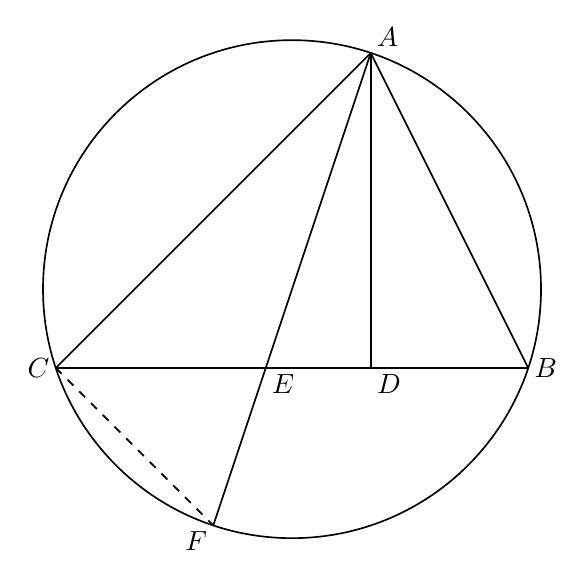
\begin{tikzpicture}[x=1cm,y=1cm,line width=.6pt,font=\normalsize]
\coordinate (O) at (0,1);
\coordinate (A) at (1,4);
\coordinate (C) at (-3,0);
\coordinate (B) at (3,0);
\coordinate (D) at (1,0);
\coordinate (E) at (-0.3333333333,0);
\coordinate (F) at (-1,-2);
\draw (O) circle[radius=3.1622776602cm];
\draw (A)--(C);
\draw (A)--(B);
\draw (C)--(B);
\draw (A)--(D);
\draw (A)--(F);
\draw[dashed] (C)--(F);
\node[above right=2pt,inner sep=0pt] at (A) {$A$};
\node[right=2pt,inner sep=0pt] at (B) {$B$};
\node[left=2pt,inner sep=0pt] at (C) {$C$};
\node[below right=2pt,inner sep=0pt] at (D) {$D$};
\node[below right=2pt,inner sep=0pt] at (E) {$E$};
\node[below left=2pt,inner sep=0pt] at (F) {$F$};
\end{tikzpicture}
